\section{Live Sanitization}
\label{sec:sanitization}

\begin{figure}[t]
  \begin{center}
    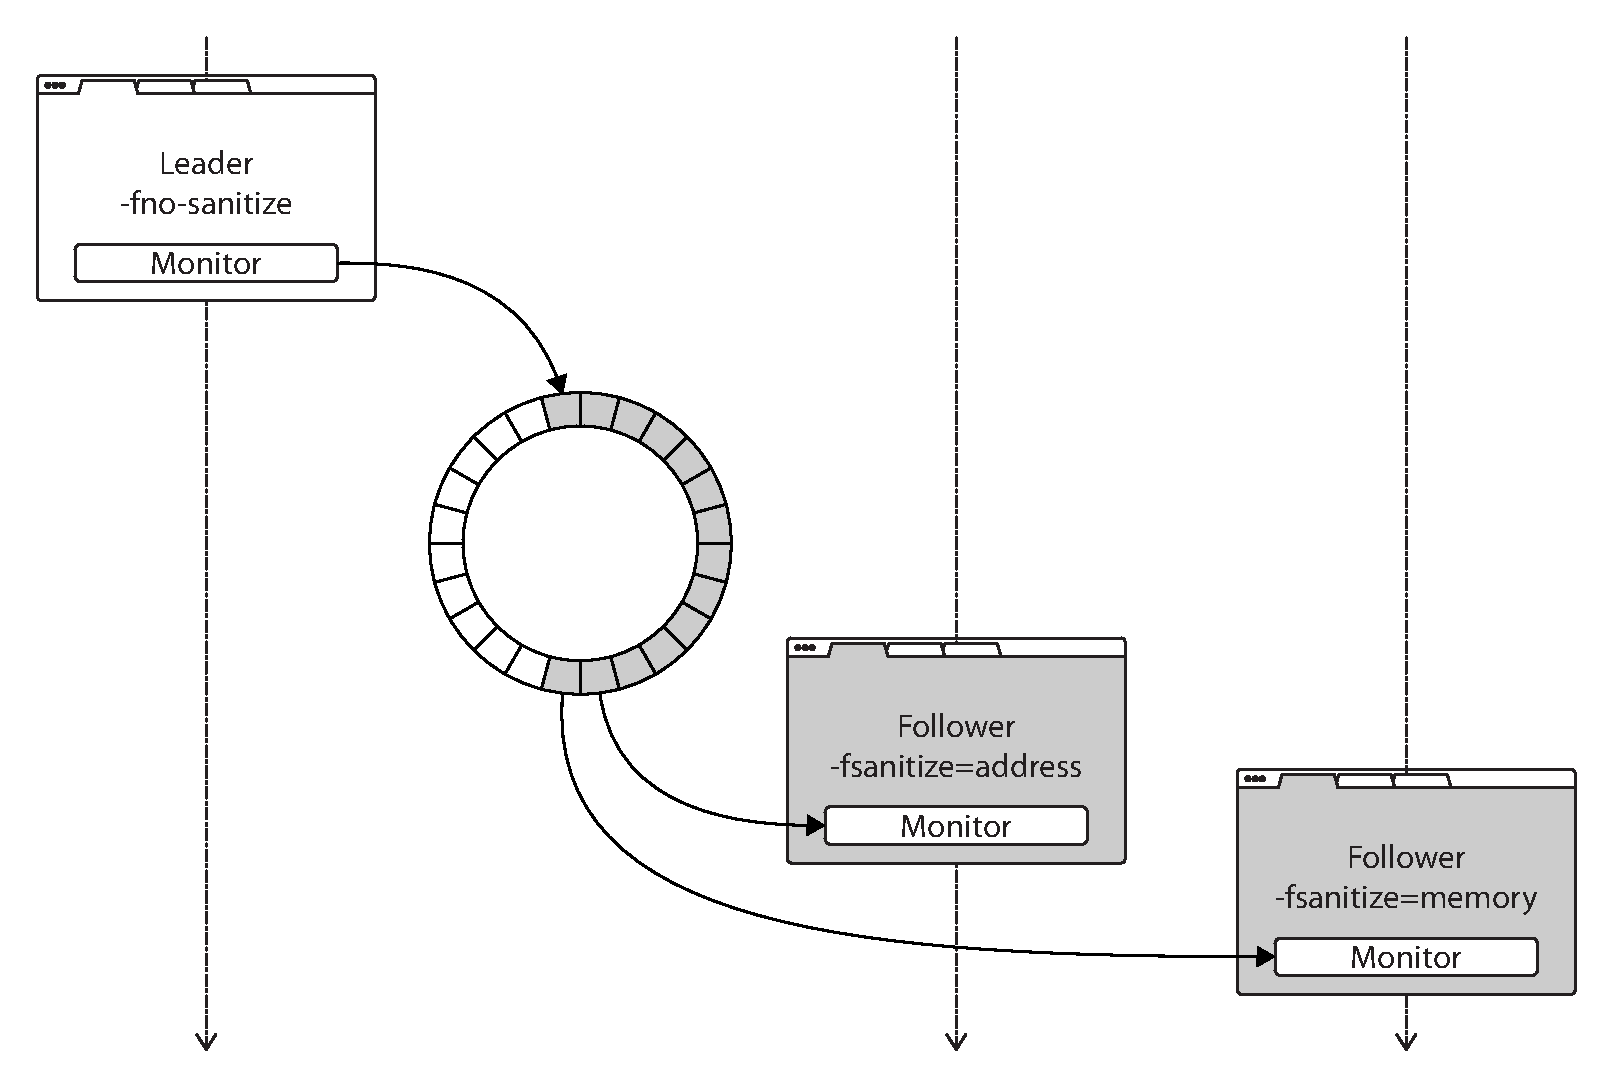
\includegraphics[width=0.75\columnwidth]{applications/figures/live-sanitization}
    \caption{The use of event-streaming architecture for live sanitization.}
    \label{fig:live-sanitization}
  \end{center}
\end{figure}

Sanitization is one of the most effective testing techniques for
revealing low-level bugs such as uninitialized pointer dereferences and
use-after-free errors.  Both Clang and GNU C Compiler now include a set
of sanitizers---AddressSanitizer (ASan), MemorySanitizer (MSan),
ThreadSanitizer (TSan)---which can be used to statically instrument
the code with various checks.  Unfortunately, these checks introduce
extra overhead (\eg $~2\times$ for ASan, $~3\times$ for MSan and
$~5$-$15\times$ for TSan).  which is why these sanitizers are typically
only used in off-line testing. However, during testing developers only
use a limited set of inputs which might not reveal all bugs.

One possible solution is to record execution traces during deployment
and then replay them in a testing environment with sanitization
enabled. However, this approach is unlikely to work in practice for
several reasons. First, since we do not know in advance which traces
are potentially interesting (\eg trigger sanitization checks) and
which are not, we have to potentially collect and replay a huge number
of execution traces. Even with some form of deduplication, this is
usually impractical. Second, for long-running applications such as
servers, the log size will quickly grow to a large size. Third, many
customers will refuse to share the logs from their production
deployment.
% While we may attempt to anonymize these logs, this could
% potentially hide interesting cases.

With \varan, we can perform live sanitization by running the native
unsanitized version as the leader, with sanitized versions as
followers.%, as shown in Figure~\ref{fig:live-sanitization}.
While sanitization itself introduces a performance overhead, since
followers do not need to execute any I/O operations and merely replay
them, they can often keep up with the leader, allowing users to run
sanitized versions in production without introducing any significant
overhead.

To demonstrate this, we build revision \lstinline`7f77235` of \redis
twice: once with Clang without any sanitization, once with ASan
enabled.  We then ran both versions in parallel using \varan and used
the same benchmark with the same settings as for our performance
evaluation (\S\ref{sec:c10k}). As expected, we have not measured any
additional slowdown in the leader compared to the scenario with two
non-sanitized versions being run in parallel. To get a better insight
into the effect of running the sanitized version with \varan, we have
measured the median length of the log, \ie the distance between the
leader and the follower. With sanitization, this length increases from
\redisNoSanitizationMedianLength to \redisSanitizationMedianLength,
which does not impose any problems.
